 \documentclass[5]{article}
\usepackage[utf8]{inputenc}
\usepackage{hyperref} 

\usepackage[T1]{fontenc}
\usepackage[polish]{babel}

\title{Laboratorium 7}
\author{Piotr Witek}
\date{5 maja 2021}

\usepackage{natbib}
\usepackage{graphicx}
\usepackage{geometry}
\usepackage{tabularx}
\usepackage{array}
\usepackage{amsmath}

\begin{document}

\newgeometry{tmargin=2cm, bmargin=2cm, lmargin=2.5cm, rmargin=2.5cm}

\maketitle


\section{Zadanie}

\hspace{4mm} Korzystając z przykładowego programu, dostarczonego wraz z poleceniem, napisałem program rozwiązujący układ równań trzema sposobami: 
\begin{enumerate}
    \item poprzez  dekompozycję LU macierzy A: A=LU
    \item poprzez odwrócenie macierzy A: x=A-1 b
    \item poprzez dekompozycję QR macierzy A: A=QR
\end{enumerate}

Argumentem wejściowym programu jest liczba naturalna, będąca rozmiarem układu równań. Program umożliwia ponadto zmierzenie czasu wykonania dla każdej z wyżej wymienionych operacji.

\vspace{4mm}
Aby sprawdzić poprawność działania programu wykonałem test na przykładowych danych:

\begin{center}
    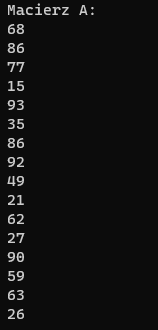
\includegraphics[scale=0.8]{przyklad_A.PNG} \par
    \vspace{3mm}
\end{center}
\hfil{Rysunek 1: Macierz A przykładowych danych} \par

\begin{center}
    \vspace{4mm}
    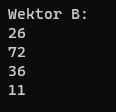
\includegraphics[scale=0.8]{przyklad_B.PNG} \par
\end{center}
\hfil{Rysunek 2: Macierz B przykładowych danych} \par

\vspace{4mm}
Następnie porównałem wyniki każdej z trzech metod, wszystkie okazały się tożsame:

\begin{center}
    \vspace{4mm}
    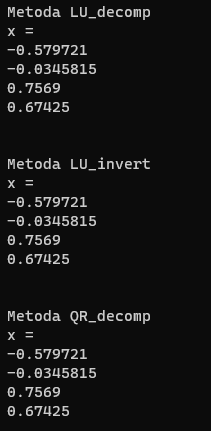
\includegraphics[scale=0.8]{przyklad_x.PNG} \par
\end{center}
\hfil{Rysunek 3: Wyniki operacji na macierzach A i B dla każdej z metod} \par


\section{Zadanie domowe}


\hspace{4mm} W ramach tego zadania wykonałem analizę całkowitego czasu wykonania każdej z trzech operacji dla 5 wartości z przedziału [10,100]:


\begin{center}
    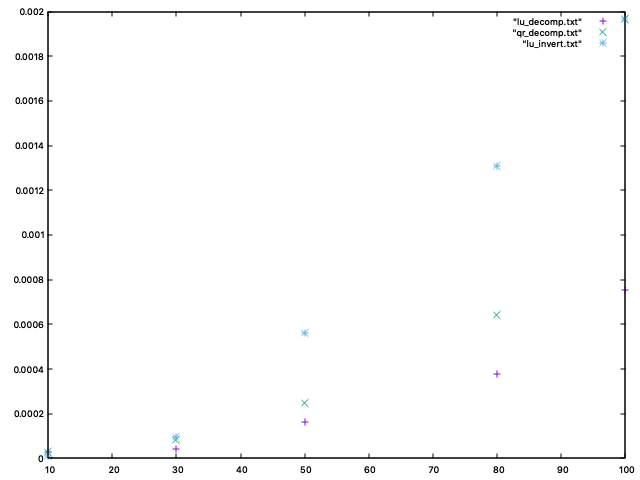
\includegraphics[scale=0.6]{porównanie.png} \par
    \vspace{3mm}
\end{center}


\section{Wnioski}
Z przeprowadzonego eksperymetu wynika, że najszybsza metodą jest dekompozycja LU, troszkę wolniejszą jest dekompozycja QR, a najwolniejszą odwracanie macierzy.

\section{Bibliografia}

\begin{enumerate}
  \item \url{https://pl.wikipedia.org/wiki/Metoda_LU}
  \item \url{https://pl.wikipedia.org/wiki/Rozk%C5%82ad_QR}
  \item \url{https://www.gnu.org/software/gsl/doc/html/vectors.html}
  \item \url{https://www.gnu.org/software/gsl/doc/html/blas.html}
\end{enumerate}

\end{document}

